\section{Aufbau und Durchführung}
\label{sec:Durchführung}
\subsection{Aufbau}

In der Mitte einer Billiardkugel befindet sich ein Permanentmagnet. Sein magnetisches Moment zeigt in Richtung des Stiels. Die Kugel bewegt sich,wegen eines Luftkissens,reibungsfrei auf einem Messingzylinder, zwischen zwei Helmholtz-Spulen.  Die zwei Helmholtz-Spulen (N=195) erzeugen ein Magnetfeld, und haben einen Abstand von d = 0.138 m und einen Radius von R = 0.109 m.
Ein Stroboskop, welches sich an der oberen Spule befindet, bestimmt die Drehbewegung.
Mit einem Steuergerät können Strom, Magnetfeld, Stroboskop und Luftkissen eingestellt und bedient werden.

\begin{figure}[H]
  \centering
  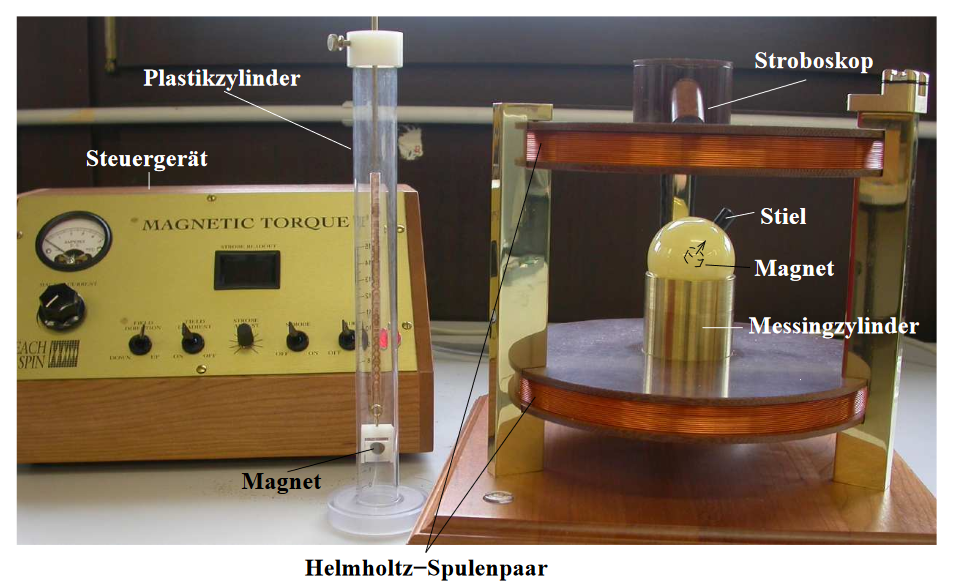
\includegraphics[height=8cm]{Screenshot (3).png}
  \caption{Versuchsaufbau}
  \label{fig:drill}
\end{figure}


\subsection{Durchführung}
Als erstes werden Radius und Masse der Billiardkugel gemessen und daraus das Trägheitsmoment bestimmt. Desweiteren wird die Länge des Stiels gemessen.

\subsubsection{Bestimmung des magnetischen Moments durch Gravitation}
In den Stiel der Kugel wird eine Aluminiumstange, auf welcher eine verschiebbare Masse ist, gesetzt, und die Kugel wird auf den Zylinder gesetzt.
Dann wird der Abstand r von Anfang des Stiels, bis Schwerpunkt der Masse, bestimmt. 
Nun wird am Steuergerät das Gebläse für das Luftkissen angeschaltet, die Feldrichtung auf ``up'' und der Feldgradient auf ``off'' gestellt.
Das Magnetfeld wird nun solange eingestellt, bis das System in einem Gleichgewicht ist. 
Ist dies der Fall, werden sich Magnetfeld und Abstand notiert.
Diese Messung wird 10 mal wiederholt, wobei der Abstand beliebig geändert wird.

\begin{figure}[H]
  \centering
  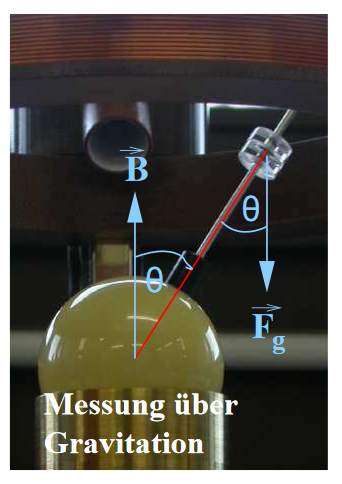
\includegraphics[height=5cm]{Screenshot (4)}
  \caption{Krafteinwirkungen.}
  \label{fig:drill}
\end{figure}


\subsubsection{Bestimmung des magnetischen Momens durch Schwingungsdauer}

Wieder wird die Kugel auf den Zylinder gesetzt und das Magnetfeld eingeschaltet.
Die Kugel wird bei eingestelltem Magnefeld nun in Schwingung versetzt, in dem der Stiel um einen kleinen Winkel ausgelenk wird.
Es werden 10 Perioden gemessen und die Ergebnisse gemittelt. Insgesamt wird dies für 10 Stromstärken wiederholt.


\subsubsection{Bestimmung des magnetischen Moments durch Präzession}

Es wird am Stroboskop eine Frequenz zwischen 4 und 6 Hertz eingestellt.
Die sich auf dem Zylinder befindende Kugel wird in Rotation versetzt und durch gezielte Berührungen ausgelenkt, bis sie die eingestellte Frequenz erreicht.
Dies ist der Fall, wenn der weiße Punkt auf dem Stiel stationär erscheint.
Anschliessend wird das Magnetfeld eingeschaltet und die Umlaufzeit gemessen.
Insgesamt wird dies für 10 Magnetfeldstärken durchgeführt.


\begin{figure}[H]
  \centering
  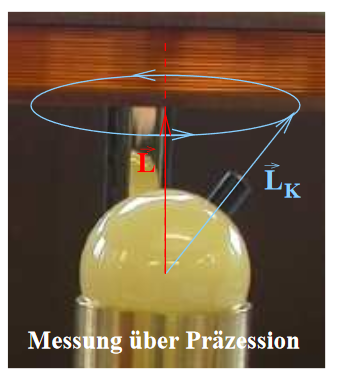
\includegraphics[height=5cm]{Screenshot (5).png}
  \caption{Achsenanordnung.}
  \label{fig:drill}
\end{figure}